\section{前期准备}
项目的前期准备主要包括天河二号实验平台的搭建和当前行人重识别领域state-of-the-art的复现。
\subsection{天河二号实验平台的搭建}

\subsubsection{天河二号实验平台参数}

天河二号拥有约17920个计算节点,每个通用节点配备两颗Xeon E5系列12核心的中央处理器、三个Xeon
Phi 57核心的协处理器(运算加速卡),总内存容量约1.4PB,全局存储总容量约12.4PB
\cite{tianhe2018config}。2017年9月,天河二号启动升级工程,二期系统天河二号A采用国产加速器
Matrix 2000,替换原有的Xeon Phi 57加速器,升级后系统峰值运算速度将达到94.97Pflops
\cite{tianhe2017summary}。天河二号各分区的详细配置如表\ref{tab:tianheconfig}。

本项目使用了天河二号的GPU分区,与其它分区最大的不同在于GPU分区每个节点都配备了2块NVIDIA
Tesla K80显示卡,显示内存VRAM为24GB,单精度浮点数运算速度为 8.74 TFLOPS,双精度浮点数的运
算速度为 2.91 TFLOPS。每个节点同时具备高性能的CPU和GPU运算能力,方便进行深度神经网络模型训练
的对比测试。与此同时,各节点之间通过千兆网络进行连接,可用于搭建多节点分布式计算网络。

天河二号的节点分为登陆节点和计算节点。登陆节点主要用于代码编译、数据解压、环境配置等工作。计算
节点配备了高性能的CPU和GPU,主要用于大数据计算,以及大规模的编译任务。登陆节点和计算节点的操
作系统均为 CentOS 7,系统使用slurm作业管理系统管理作业队列,使用module管理各种可选的软件包、
运行库。

\subsubsection{软件编译安装}

由于天河二号的登陆节点和计算节点均不能连接互联网,同时普通用户也没有直接安装软件的权限,
所以需要将必要的软件先在本地完成安装,再通过FTP协议将二进制文件打包传输到天河二号上。

由于需要复现的模型在结构上比较独特,训练方式也千奇百怪。对于 Caffe 和 TensorFlow 这样的
预编译框架,不灵活这一缺陷就变得十分明显了。

而这方面正是 PyTorch 的强项,它是一个非常 Pythonic 的深度学习框架,一切的操作(包括模型
的定义、训练、测试)都十分地符合 Python 的简单的哲学,可以非常轻松快速地构建出一个十分怪
异的模型,非常适合科研人员。

\subsubsection{安装Anaconda}

安装Anaconda十分简单,只需要从官网上下载相应平台的安装包,直接执行安装即可。

\subsubsection{安装CUDA和cuDNN}

CUDA采用最新的9.0版本,直接从NVIDIA官网下载安装即可。cuDNN需要注册开发者账户并填写问卷
即可下载安装。

\subsubsection{安装PyTorch}

在Anaconda里创建独立的Python3 env,然后执行
conda install pytorch torchvision cuda90 -c pytorch 即可。

\begin{table}[]
\centering
\caption{天河二号各分区配置表:天河二号的节点分别属于三个分区:CPU分区、GPU分区和胖节点分区。
其中CPU分区内的节点数量最多,是天河二号的计算主力,每个节点配备了2块12核的Intel Xeon E5-2692
处理器以及64GB内存,既能通过分布式联合满足大型计算的需求,又能保持在小型计算中节能的优势。GPU
分区的特点是每个节点配备了2块NVIDIA Tesla K80显示卡,每张显示卡的VRAM为24GB,同时节点的通
用RAM为256GB,可以很好地满足大量图像处理、图形渲染的需求。胖节点分区的节点配备了足够大的内存,
同时对于CPU也进行了升级,满足特定计算场景下的特殊需求。}

\label{tab:tianheconfig}
\begin{tabular}{|c|c|c|c|c|}
\hline
\multicolumn{2}{|c|}{节点/分区}  & CPU                          & 内存    & GPU                  \\ \hline
\multicolumn{2}{|c|}{CPU分区}  & 2 $\times$ 12 Intel Xeon E5-2692 v2 & 64GB  & -                    \\ \hline
\multicolumn{2}{|c|}{GPU分区}  & 2 $\times$ 10 Intel Xeon E5-2660 v3 & 256GB & 2 $\times$ NVIDIA Tesla K80 \\ \hline
\multirow{3}{*}{胖节点} & 128GB & 2 $\times$ 12 Intel Xeon E5-2692 v2 & 128GB & -                    \\ \cline{2-5}
                     & 3TB   & 4 $\times$ 14 Intel Xeon E7-4850 v3 & 3TB   & -                    \\ \cline{2-5}
                     & 6TB   & 8 $\times$ 16 Intel Xeon E7-8867 v3 & 6TB   & -                    \\ \hline
\end{tabular}
\end{table}

\subsection{数据采集}

要研究摄像头的数量与部署位置对行人重识别算法的影响,数据集需要满足以下要求:一、数据集中摄像头的个数需要超过10个,以便控制增减摄像头的进行分析对比,分析摄像头的拍摄位置对于监控效果的影响;二、存在视野重叠或拍摄位置接近的摄像头,以便分析同一位置、不同拍摄角度的拍摄方案对于监控效果的影响。三、行人需要出现在多个(而不仅仅是两个)摄像头画面内,且摄像头的分布呈路线状(可以存在分支),这样更符合行人跟踪的定义,更好地评估摄像头部署位置的监控效果。

表\ref{tab:reiddataset}是对当前行人重识别领域常见数据库的统计。从表中可以看到在当前主流数据中,VIPeR\cite{gray2007evaluating}、CUHK01\cite{li2012human}、Market1501\cite{zheng2015scalable}和DukeMTMC-reID\cite{ristani2016MTMC}数据集中摄像头数量较少,不利于分析增减摄像头以评估摄像头数量对监控效果的影响。包括CUHK03\cite{li2014deepreid}在内的所有数据集都缺乏单个行人持续追踪的场景,不利于实现监控效果的评估。

因此,有必要针对上述需求重新采集一个数据库,满足研究和实验的需求。经过路线规划、场地布置、演员召集等工作,目前完成了数据库的预拍摄工作。数据集的正式拍摄计划与2018年5月18日和19日进行,计划召集500余名演员参与。第一次预拍摄过程的详细情况如下:

第一次拍摄的参与者为 19 人,其中有 15 人完整地走完了路线,全程拍摄时长大约为 25 分钟。视频拍摄的地点位于中山大学数据科学与计算机学院楼外停车场与楼内1、2、3、4、6楼的大厅和走廊。视频拍摄过程中需要在若干个关键点(某个摄像头或者某一楼层)设置人员负责时间点记录和人流控制,记下每一个演员进入视频画面的时间点,用于之后的视频分割。

本次拍摄一共使用了 21 个摄像头,最终 20 个摄像头有视频输出。其中原有的摄像头个数为 14 个,新增 DV 5 台,其中有 1 台不能正常写入视频文件,新增手机 2 部。原有的监控视频的分辨率大部分为 1280$\times$720(720P),也有部分是 1920$\times$1080(1080P),新增的 DV 拍摄的视频分辨率都是 1080P,新增的 2 部手机的分辨率分别为 720P 和 1080P。视频的帧率均为 25 FPS。

最终用于本项目的数据集包含17个摄像头的视频数据,每个摄像头的视频数据包含在一个视频文件内,视频的长度约为10分钟,出现的演员有15人。

\begin{table}[]
\centering
\caption{行人重识别领域常见数据库情况统计}
\label{tab:reiddataset}
\begin{threeparttable}
\begin{tabular}{|c|c|c|c|c|c|c|}
\hline
数据集名称         & 公布时间 & 行人数量 & 摄像头数量 & 图片数量  & Multi-shot\tnote{*} & Tracking\tnote{**} \\ \hline
VIPeR         & 2007 & 632  & 2     & 1264  & 否          & 否                  \\ \hline
CUHK01        & 2012 & 971  & 2     & 3884  & 否          & 否                  \\ \hline
CUHK03        & 2014 & 1467 & 10    & 13164 & 是          & 否                  \\ \hline
Market1501    & 2015 & 1501 & 6     & 32217 & 是          & 否                  \\ \hline
DukeMTMC-reID & 2017 & 1812 & 8     & 36441 & 是          & 否                  \\ \hline
\end{tabular}
\begin{tablenotes}
    \footnotesize
    \item[*] 同一行人是否有超过2张图片。
    \item[**] 是否持续追踪同一行人。
\end{tablenotes}
\end{threeparttable}
\end{table}

\begin{figure}
\centering
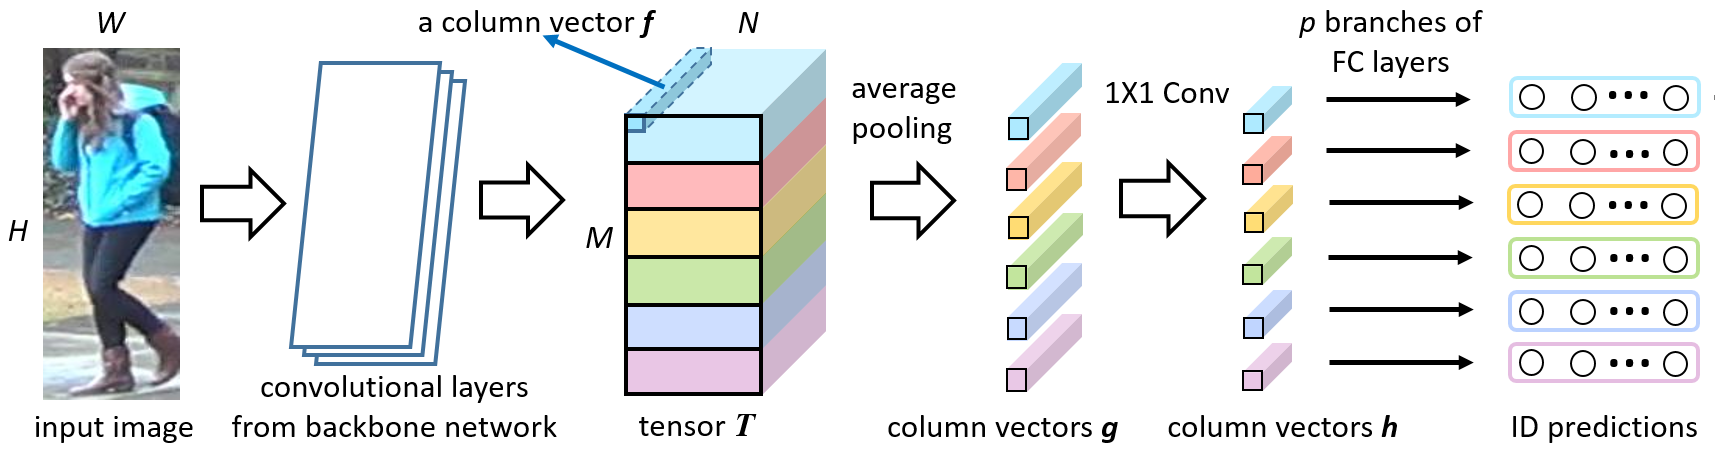
\includegraphics[width=1\textwidth]{figure/structure}
\caption{Baseline架构图}
\label{fig:baseline}
\end{figure}
